\ifdissForPrint
\iflicense
\newpage
\thispagestyle{empty}

\vspace*{\fill} 

\noindent
\begin{minipage}[b]{\textwidth}

\ifsharealike

\includegraphics[scale=1]{License/by-sa.eps}\\
 
\ifenglish
\textit{This document - excluding the cover, pictures, tabels and graphs - is licensed under the Creative Commons Attribution-ShareAlike 4.0 International License (CC BY-SA 4.0): https://creativecommons.org/licenses/by-sa/4.0/}

\else
\textit{Dieses Werk - ausgeschlossen der Einband, Abbildungen, Tabellen und Graphen - ist lizenziert unter einer Creative Commons Namensnennung - Weitergabe unter gleichen Bedingungen 4.0 Internationalen Lizenz (CC BY-SA 4.0): https://creativecommons.org/licenses/by-sa/4.0/}
\fi

\else

\includegraphics[scale=1]{License/by-nc-nd.eps}\\

\ifenglish
\textit{This document - excluding the cover, pictures, tabels and graphs - is licensed under the Creative Commons Attribution-NonCommercial-NoDerivs 4.0 International License (CC BY-NC-ND 4.0): https://creativecommons.org/licenses/by-nc-nd/4.0/}

\else
\textit{Dieses Werk - ausgeschlossen der Einband, Abbildungen, Tabellen und Graphen - ist lizenziert unter einer Creative Commons Namensnennung - Nicht-kommerziell - Keine Bearbeitung 4.0 Internationalen Lizenz (CC BY-NC-ND 4.0): https://creativecommons.org/licenses/by-nc-nd/4.0/}
\fi
\fi

\end{minipage}
\fi

\else
\thispagestyle{empty}
\afterpage{\newpage}
\fi

%The license text can be restricted or generalized for some single chapters or what ever you want.
%All the followed License types are stored in the license folder an can be used, but the curent link in the discription must be changed.


%The Licenses
%more information under https://creativecommons.org/licenses/
%
%Attribution 
%CC BY
%
%This license lets others distribute, remix, tweak, and build upon your work, even commercially, as long as they credit you for the original creation. This is the most accommodating of licenses offered. Recommended for maximum dissemination and use of licensed materials.
%
%View License Deed | View Legal Code
%
%
%Attribution-ShareAlike 
%CC BY-SA
%
%This license lets others remix, tweak, and build upon your work even for commercial purposes, as long as they credit you and license their new creations under the identical terms. This license is often compared to “copyleft” free and open source software licenses. All new works based on yours will carry the same license, so any derivatives will also allow commercial use. This is the license used by Wikipedia, and is recommended for materials that would benefit from incorporating content from Wikipedia and similarly licensed projects.
%
%View License Deed | View Legal Code
%
%
%Attribution-NoDerivs 
%CC BY-ND
%
%This license allows for redistribution, commercial and non-commercial, as long as it is passed along unchanged and in whole, with credit to you.
%
%View License Deed | View Legal Code
%
%
%Attribution-NonCommercial 
%CC BY-NC
%
%This license lets others remix, tweak, and build upon your work non-commercially, and although their new works must also acknowledge you and be non-commercial, they don’t have to license their derivative works on the same terms.
%
%View License Deed | View Legal Code
%
%
%Attribution-NonCommercial-ShareAlike 
%CC BY-NC-SA
%
%This license lets others remix, tweak, and build upon your work non-commercially, as long as they credit you and license their new creations under the identical terms.
%
%View License Deed | View Legal Code
%
%
%Attribution-NonCommercial-NoDerivs 
%CC BY-NC-ND
%
%This license is the most restrictive of our six main licenses, only allowing others to download your works and share them with others as long as they credit you, but they can’t change them in any way or use them commercially.
